\documentclass[border=5pt]{standalone}
\usepackage{tikz}
\usetikzlibrary{arrows.meta, positioning}
\usepackage{xcolor}

\definecolor{Garnet}{HTML}{73000A}
\definecolor{NinetyBlack}{HTML}{363636}
\definecolor{SeventyBlack}{HTML}{5C5C5C}
\definecolor{FiftyBlack}{HTML}{A2A2A2}
\definecolor{ThirtyBlack}{HTML}{C7C7C7}
\definecolor{TenBlack}{HTML}{ECECEC}
\definecolor{Atlantic}{HTML}{466A9F}
\definecolor{Rose}{HTML}{CC2E40}
\definecolor{Congaree}{HTML}{1F414D}

\tikzset{every node/.append style={rounded corners=0pt}}

\begin{document}
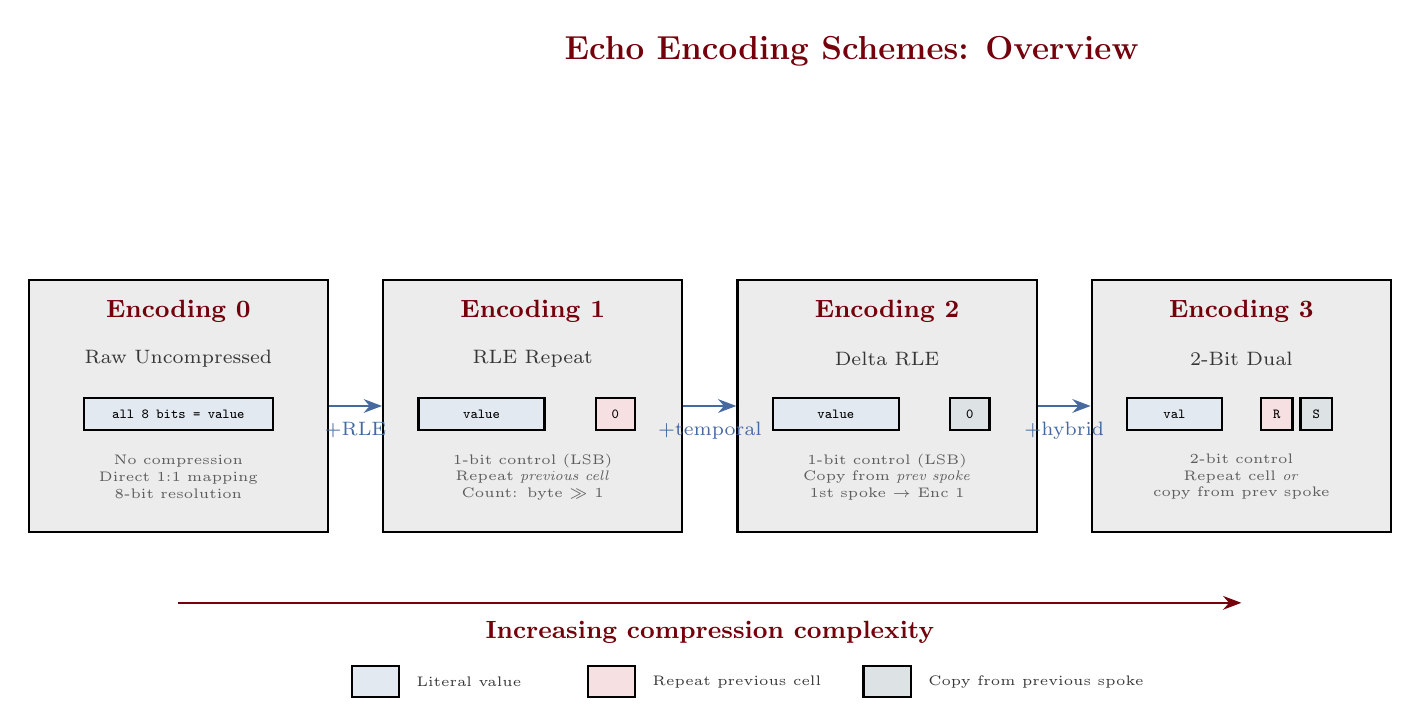
\begin{tikzpicture}[
    enc/.style={draw, thick, minimum width=3.8cm, minimum height=3.2cm, align=center, fill=TenBlack, inner sep=5pt},
    elbl/.style={font=\small\bfseries, color=Garnet},
    sub/.style={font=\scriptsize, color=NinetyBlack},
    ctrl/.style={draw, thick, minimum height=0.4cm, font=\tiny\ttfamily\bfseries},
]

% Title
\node[font=\bfseries\large, color=Garnet] at (8.55, 4.5) {Echo Encoding Schemes: Overview};

% Encoding 0
\node[enc] (e0) at (0, 0) {};
\node[elbl] at (0, 1.2) {Encoding 0};
\node[sub] at (0, 0.6) {Raw Uncompressed};
\node[ctrl, fill=Atlantic!15, minimum width=2.4cm] at (0, -0.1) {all 8 bits = value};
\node[font=\tiny, color=SeventyBlack, text width=3cm, align=center] at (0, -0.9) {No compression\\Direct 1:1 mapping\\8-bit resolution};

% Encoding 1
\node[enc] (e1) at (4.5, 0) {};
\node[elbl] at (4.5, 1.2) {Encoding 1};
\node[sub] at (4.5, 0.6) {RLE Repeat};
\node[ctrl, fill=Atlantic!15, minimum width=1.6cm] at (3.85, -0.1) {value};
\node[ctrl, fill=Rose!15, minimum width=0.5cm] at (5.55, -0.1) {0};
\node[font=\tiny, color=SeventyBlack, text width=3cm, align=center] at (4.5, -0.9) {1-bit control (LSB)\\Repeat \textit{previous cell}\\Count: byte $\gg$ 1};

% Encoding 2
\node[enc] (e2) at (9, 0) {};
\node[elbl] at (9, 1.2) {Encoding 2};
\node[sub] at (9, 0.6) {Delta RLE};
\node[ctrl, fill=Atlantic!15, minimum width=1.6cm] at (8.35, -0.1) {value};
\node[ctrl, fill=Congaree!15, minimum width=0.5cm] at (10.05, -0.1) {0};
\node[font=\tiny, color=SeventyBlack, text width=3cm, align=center] at (9, -0.9) {1-bit control (LSB)\\Copy from \textit{prev spoke}\\1st spoke $\rightarrow$ Enc 1};

% Encoding 3
\node[enc] (e3) at (13.5, 0) {};
\node[elbl] at (13.5, 1.2) {Encoding 3};
\node[sub] at (13.5, 0.6) {2-Bit Dual};
\node[ctrl, fill=Atlantic!15, minimum width=1.2cm] at (12.65, -0.1) {val};
\node[ctrl, fill=Rose!15, minimum width=0.4cm] at (13.95, -0.1) {\tiny R};
\node[ctrl, fill=Congaree!15, minimum width=0.4cm] at (14.45, -0.1) {\tiny S};
\node[font=\tiny, color=SeventyBlack, text width=3cm, align=center] at (13.5, -0.9) {2-bit control\\Repeat cell \textit{or}\\copy from prev spoke};

% Arrows between boxes
\draw[-{Stealth}, thick, color=Atlantic] (e0) -- (e1)
    node[midway, below=2pt, font=\scriptsize, color=Atlantic] {+RLE};
\draw[-{Stealth}, thick, color=Atlantic] (e1) -- (e2)
    node[midway, below=2pt, font=\scriptsize, color=Atlantic] {+temporal};
\draw[-{Stealth}, thick, color=Atlantic] (e2) -- (e3)
    node[midway, below=2pt, font=\scriptsize, color=Atlantic] {+hybrid};

% Bottom annotation
\draw[-{Stealth}, thick, color=Garnet] (0, -2.5) -- (13.5, -2.5)
    node[midway, below=3pt, font=\small\bfseries, color=Garnet] {Increasing compression complexity};

% Control bit legend
\node[ctrl, fill=Atlantic!15, minimum width=0.6cm] at (2.5, -3.5) {};
\node[font=\tiny, color=NinetyBlack, anchor=west] at (2.9, -3.5) {Literal value};
\node[ctrl, fill=Rose!15, minimum width=0.6cm] at (5.5, -3.5) {};
\node[font=\tiny, color=NinetyBlack, anchor=west] at (5.9, -3.5) {Repeat previous cell};
\node[ctrl, fill=Congaree!15, minimum width=0.6cm] at (9.0, -3.5) {};
\node[font=\tiny, color=NinetyBlack, anchor=west] at (9.4, -3.5) {Copy from previous spoke};

\end{tikzpicture}
\end{document}
